\documentclass{article}
\usepackage{graphicx}
\usepackage{tikz}
\usepackage{amsmath}
\usepackage{hyperref}
\usepackage[a4paper, margin=2.5cm]{geometry}
\setlength{\parindent}{0pt} % Set paragraph indentation to zero

\begin{document}

\section*{Neuron}

Schema of a neuron:
\begin{center}
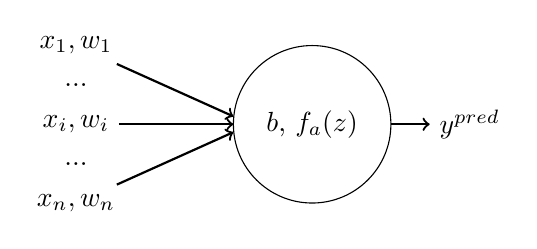
\begin{tikzpicture}
  % Draw a circle with radius 1
  \draw (3,2) circle (1);
  \node[black] at (3,2) {$b$, $f_a(z)$};
  \node[black] (x1) at (0,3) {$x_1, w_1$};
  \draw[->, thick] (x1) -- (2,2.1);
  \node[black] at (0,2.5) {...};
  \node[black] (xi) at (0,2) {$x_i, w_i$};
  \draw[->, thick] (xi) -- (2,2);
  \node[black] at (0,1.5) {...};
  \node[black] (xn) at (0,1) {$x_n, w_n$};
  \draw[->, thick] (xn) -- (2,1.9);
  \node[black] (out) at (5,2) {$y^{pred}$};
  \draw[->, thick] (4,2) -- (out);
\end{tikzpicture}
\end{center}

To compute predicted value by the neuron:
\begin{equation}
  z = \sum_{i=1}^n w_ix_i + b
\end{equation}

\begin{equation}
  y^{pred} = f_a(z) = f_a(\sum_{i=1}^n w_ix_i + b)
\end{equation}

To compute the cost function for $m$ training samples:
\begin{align}
  C(w,b) &= \frac{1}{2m} \sum_{j=1}^m \left(y_j^{pred} - y_j\right)^2 \nonumber \\
         &= \frac{1}{2m} \sum_{j=1}^m \left(f_a(z)_j - y_j\right)^2
\end{align}

Training the neuron consists on minimizing the cost function. The method used to minimize the cost function is Gradient Descent (\url{https://en.wikipedia.org/wiki/Gradient_descent}).

\begin{align}
  \mathbf{w}^{n+1} &= \mathbf{w}^n - \alpha \nabla C(\mathbf{w}^n, b^n) \\
  b^{n+1} &= b^n - \alpha \nabla C(\mathbf{w}^n, b^n)
\end{align}

The equations above compute the gradient descent for the weights and for the bias. $\alpha$ is the so called Learning Rate.

To compute the gradient of the cost function for $m$ training samples, it is necessary to compute the partial derivatives with respect $\mathbf{w}$ and $b$.

Partial derivative with respect $\mathbf{w}$:
\begin{align}
  \dfrac{\delta C(\mathbf{w},b)}{\delta w_i}
  &= \left( \frac{1}{2m} \left(f_a(z) - y\right)^2 \right)' \nonumber \\
  &= \frac{1}{m} \left(f_a(z) - y\right) f_a'(z) z' \nonumber \\
  &= \frac{1}{m} \sum_{j=1}^m \left(f_a(\mathbf{w^T \cdot x} + b) - y_j\right) f_a'(\mathbf{w^T \cdot x} + b) (x_i)_j
\end{align}

In a similar way, the partial derivative with respect $b$:
\begin{equation}
  \dfrac{\delta C(\mathbf{w},b)}{\delta b} = \frac{1}{m} \sum_{j=1}^m \left(f_a(\mathbf{w^T \cdot x} + b) - y_j\right) f_a'(\mathbf{w^T \cdot x} + b)
\end{equation}

\section*{Activation functions}

\subsection*{Sigmoid}

Sigmoid function is:
\begin{equation}
  \sigma(x) = \frac{1}{1 + e^{-x}}
\end{equation}

Sigmoid derivative is:
\begin{equation}
  \sigma'(x) = \sigma(x) \cdot (1 - \sigma(x))  
\end{equation}

\subsection*{ReLU}

ReLU function is:
\begin{equation}
  ReLU(x) = \max(0,x)
\end{equation}

The derivative of the ReLU function is:
\begin{equation}
  ReLU'(x) = \begin{cases} 
    0 & x < 0 \\
    1 & x\geq 0 
  \end{cases}
\end{equation}

\section*{Network}
\begin{center}
  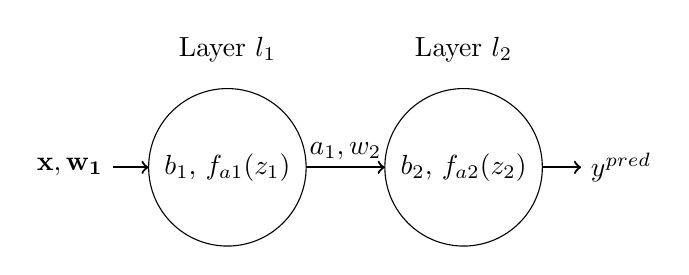
\begin{tikzpicture}
    % Draw Layer 1
    \node[black] at (3,3.5) {Layer $l_1$};
    \draw (3,2) circle (1);
    \node[black] at (3,2) {$b_1$, $f_{a1}(z_1)$};
    \node[black] (x) at (1,2) {$\mathbf{x}, \mathbf{w_1}$};
    \draw[->, thick] (x) -- (2,2);
    \node[black] at (4.5,2.2) {$a_1, w_2$};
    \draw (6,2) circle (1);
    \draw[->, thick] (4,2) -- (5,2);
    \node[black] at (6,2) {$b_2$, $f_{a2}(z_2)$};
    \node[black] at (6,3.5) {Layer $l_2$};
    \node[black] (out) at (8,2) {$y^{pred}$};
    \draw[->, thick] (7, 2) -- (out);
  \end{tikzpicture}
\end{center}

Compute Layer 1:
\begin{align}
  z_1 &= \mathbf{w_1^T} \cdot \mathbf{x} + b_1 \nonumber \\
  a_1 &= f_{a1}(z_1) = f_{a1}(\mathbf{w_1^T} \cdot \mathbf{x} + b_1)
\end{align}

Compute Layer 2:
\begin{align}
  z_2 &= w_2 a_1 + b_2 \nonumber \\
  y^{pred} &= f_{a2}(z_2) = f_{a2}(w_2 a_1 + b_2)
\end{align}

Network:
\begin{equation}
  y^{pred} = f_{a2}(w_2 f_{a1}(\mathbf{w_1^T} \cdot \mathbf{x} + b_1) + b_2)
\end{equation}

Cost function for $m$ samples:
\begin{align}
  C(\mathbf{w^*},\mathbf{b^*}) &= \dfrac{1}{2m} \sum_{i=1}^m (y^{pred} - y)^2 \nonumber \\
  &= \dfrac{1}{2m} \sum_{i=1}^m (f_{a2}(w_2 f_{a1}(\mathbf{w_1^T} \cdot \mathbf{x} + b_1) + b_2) - y)^2
\end{align}

Derivative of the cost function:
\begin{align}
  \nabla_{\mathbf{w^*}}C(\mathbf{w^*}, \mathbf{b^*}) = [\delta_{w_1} C(\mathbf{w^*}, \mathbf{b^*}), ..., \delta_{w_i} C(\mathbf{w^*}, \mathbf{b^*}), ..., \delta_{w_n} C(\mathbf{w^*}, \mathbf{b^*})]  \\
  \nabla_{\mathbf{b^*}}C(\mathbf{w^*}, \mathbf{b^*}) = [\delta_{b_1} C(\mathbf{w^*}, \mathbf{b^*}), ..., \delta_{b_i} C(\mathbf{w^*}, \mathbf{b^*}), ..., \delta_{b_n} C(\mathbf{w^*}, \mathbf{b^*})]
\end{align}

In our case:
\begin{align}
  \nabla_{\mathbf{w^*}}C(\mathbf{w^*}, \mathbf{b^*}) = [\delta_{w_1} C(\mathbf{w^*}, \mathbf{b^*}), \delta_{w_2} C(\mathbf{w^*}, \mathbf{b^*})]  \\
  \nabla_{\mathbf{b^*}}C(\mathbf{w^*}, \mathbf{b^*}) = [\delta_{b_1} C(\mathbf{w^*}, \mathbf{b^*}), \delta_{b_2} C(\mathbf{w^*}, \mathbf{b^*})]
\end{align}

Let's define some nomencalutre before compute the gradients of the cost function:

\begin{align}
  \mathbf{a_0} &= \mathbf{x} \\ 
  z_1 &= \mathbf{w_1^T} \cdot \mathbf{x} + b_1 \\
  a_1 &= f_{a1}(z_1) = f_{a1}(\mathbf{w_1^T} \cdot \mathbf{x} + b_1) \\
  z_2 &= w_2 f_{a1}(z_1) + b_2 = w_2 f_{a1}(\mathbf{w_1^T} \cdot \mathbf{x} + b_1) + b_2 \\
  a_2 &= f_{a2}(z_2) = w_2 f_{a1}(z_1) + b_2
\end{align}

Let's compute the gradients with respect the weights $\mathbf{w^*}$:
\begin{align}
  \delta_{w_1} C(\mathbf{w^*}, \mathbf{b^*}) &= \delta_{w_1} ( \dfrac{1}{2m} \sum_{i=1}^m (a_2 - y)^2) \nonumber \\
  &= \dfrac{1}{m} \sum_1^m (a_2 - y) f'_{a2}(z_2) w_2 f'_{a1}(z_1) \mathbf{a_0} \\
  \delta_{w_2} C(\mathbf{w^*}, \mathbf{b^*}) &= \delta_{w_2} ( \dfrac{1}{2m} \sum_{i=1}^m (a_2 - y)^2) \nonumber \\
  &= \dfrac{1}{m} \sum_1^m (a_2 - y) f'_{a2}(z_2) a_1 
\end{align}

Let's do the same for the bias $\mathbf{b^*}$:
\begin{align}
  \delta_{b_1} C(\mathbf{w^*}, \mathbf{b^*}) &= \delta_{b_1} ( \dfrac{1}{2m} \sum_{i=1}^m (a_2 - y)^2) \nonumber \\
  &= \dfrac{1}{m} \sum_1^m (a_2 - y) f'_{a2}(z_2) w_2 f'_{a1}(z_1) \\
  \delta_{b_2} C(\mathbf{w^*}, \mathbf{b^*}) &= \delta_{b_2} ( \dfrac{1}{2m} \sum_{i=1}^m (a_2 - y)^2) \nonumber \\
  &= \dfrac{1}{m} \sum_1^m (a_2 - y) f'_{a2}(z_2)
\end{align}

Let's generalize, and consider the bias $b$, the component $0$ of the weights, so $\mathbf{w_i} = (w_{i0}, w_{i1}, ..., w_{in})$ and $\mathbf{a_i} = (1, a_{i1}, ..., a_{in})$:
\begin{align}
  \delta_{w_i} C(\mathbf{w}) &= \dfrac{1}{2m} \sum_{i=1}^m (a_n - y) f'_{an}(z_n) w_n f'_{an-1}(z_{n-1}) w_{n-1} ... f'_{a_i}(z_i) a_i
\end{align}

\end{document}
